\mychapter{Results}{Results}{}\label{chap:results}

\mysection{Experiment 1: STFT Features}{Experiment 1: STFT Features}\label{sec:exp-1-stft}

\begin{table}[H]
    \caption{Calibration variables chosen via highest F1 for STFT for 5 templates and 10 templates}
    \footnotesize
    \setlength{\tabcolsep}{3pt}
    \centering
    \makebox[\textwidth][c]{%
    \begin{tabular}{cccccccccc}
        \toprule
        \multirow{2}{*}{Number of Temps}
            & \multicolumn{2}{c}{Single Tones}
            & \multicolumn{2}{c}{Multi Tones}
            & \multicolumn{2}{c}{Burst Tonals} 
            & \multirow{2}{*}{Avg F1}
            & \multirow{2}{*}{Frame Length}\\
        \cmidrule(lr){2-3} \cmidrule(lr){4-5} \cmidrule(lr){6-7}
            & $F_1$ & Threshold & $F_1$ & Threshold & $F_1$ & Threshold \\
        \midrule
        5  & 0.682 & 0.2339 & 0.568 & 0.2557 & 0.796 & 0.2603 &  & 0.512\\
        10 & 0.690 & 0.2455 & 0.663 & 0.2364 & 0.697 &  0.2303 & 0.512\\
        \bottomrule
    \end{tabular}\label{tab:stft_calib_results}
    }
\end{table}

\begin{table}[H]
    \caption{Vote frac results for STFT for 5 and 10 templates}
    \footnotesize
    \setlength{\tabcolsep}{3pt}
    \centering
    \begin{tabular}{ccccc}
        \toprule
        Number of Temps & Precision & Recall & F1 & Vote Fraction\\
        \midrule
        5  &  &  &  \\
        10 &  &  &  \\
        \bottomrule
    \end{tabular}\label{tab:stft_vote_results}
\end{table}

\begin{table}[H]
    \caption{Final test results for STFT for 5 and 10 templates}
    \footnotesize
    \setlength{\tabcolsep}{3pt}
    \centering
    \begin{tabular}{ccccc}
        \toprule
        Number of Temps & Precision & Recall & F1 & Average Precision \\
        \midrule
        5  & 0.646 & 0.951 & 0.7696 & 0.850 \\
        10 & 0.593 & 0.968 & 0.7350 & 0.863 \\
        \bottomrule
    \end{tabular}\label{tab:stft_test_results}
\end{table}

\begin{figure}[H]
    \centering
    \subfloat[5 templates\label{fig:stft_5_pr}]{%
        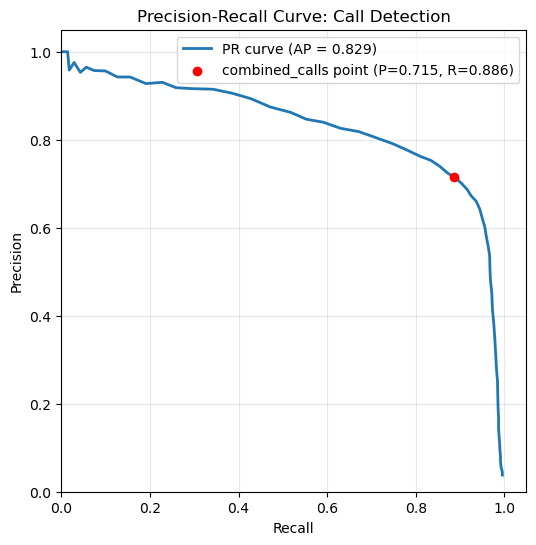
\includegraphics[width=0.3\linewidth]{figures/results/stft_5_pr.png}}
    \hspace{1cm}
    \subfloat[10 templates\label{fig:stft_10_pr}]{%
        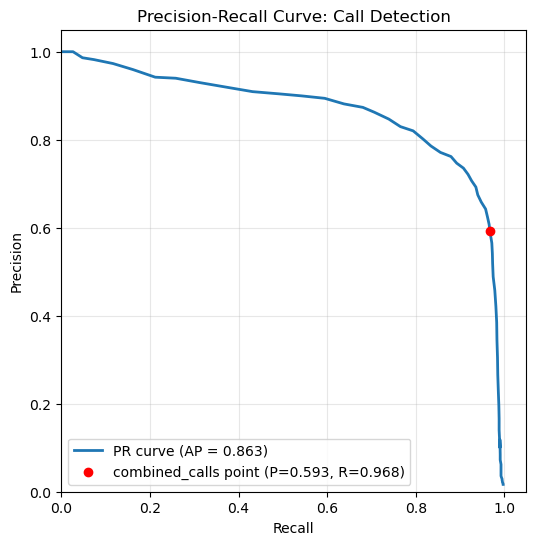
\includegraphics[width=0.3\linewidth]{figures/results/stft_10_pr.png}}
    \caption{The PR curves for STFT}\label{fig:stft_pr}
\end{figure}




\mysection{Experiment 2: MFCC Features}{Experiment 2: MFCC Features}\label{sec:exp-2-mfcc}

\begin{table}[H]
    \caption{Calibration variables chosen via highest F1 for 5 templates and 10 templates}
    \footnotesize
    \setlength{\tabcolsep}{3pt}
    \centering
    \makebox[\textwidth][c]{%
    \begin{tabular}{cccccccccc}
        \toprule
        & \multirow{2}{*}{Number of Temps}
            & \multicolumn{2}{c}{Single Tones}
            & \multicolumn{2}{c}{Multi Tones}
            & \multicolumn{2}{c}{Burst Tonals}
            & \multirow{2}{*}{Frame Length}
            & \multirow{2}{*}{Vote Fraction} \\
        \cmidrule(lr){3-4} \cmidrule(lr){5-6} \cmidrule(lr){7-8}
        & & $F_1$ & Threshold & $F_1$ & Threshold & $F_1$ & Threshold & & \\
        \midrule
        \multirow{2}{*}{MFCC}
            & 5  & 0.718 & 16.394 & 0.675 & 22.688 & 0.500 & 19.483 & 0.384 & 0.2 \\
            & 10 & 0.784 & 17.507 & 0.402 & 19.553 & 0.472 & 21.288 & 0.256 & 0.2 \\
        \midrule
        \multirow{2}{*}{\makecell{MFCC\\deriv1}}
            & 5  & 0.683 & 15.610 & 0.659 & 23.440 & 0.500 & 20.337 & 0.384 & 0.2 \\
            & 10 & 0.785 & 18.815 & 0.394 & 22.548 & 0.425 & 20.569 & 0.256 & 0.2 \\
        \midrule
        \multirow{2}{*}{\makecell{MFCC\\deriv2}}
            & 5  & 0.758 & 18.199 & 0.659 & 24.977 & 0.518 & 21.595 & 0.384 & 0.2 \\
            & 10 & 0.806 & 19.642 & 0.408 & 22.356 & 0.430 & 22.836 & 0.256 & 0.2 \\
        \bottomrule
    \end{tabular}%
    }\label{tab:mfcc_calib_results}
\end{table}

\begin{table}[H]
    \caption{Final test results for 5 and 10 templates}
    \footnotesize
    \setlength{\tabcolsep}{3pt}
    \centering
    \begin{tabular}{cccccc}
        \toprule
        & Number of Temps & Precision & Recall & $F_1$ & Average Precision \\
        \midrule
        \multirow{2}{*}{MFCC}
            & 5  & 0.063 & 0.945 & 0.117 & 0.396 \\
            & 10 & 0.108 & 0.930 & 0.194 & 0.550 \\
        \midrule
        \multirow{2}{*}{\makecell{MFCC\\deriv1}}
            & 5  & 0.141 & 0.932 & 0.246 & 0.430 \\
            & 10 & 0.030 & 0.942 & 0.0.058 & 0.0.432 \\
        \midrule
        \multirow{2}{*}{\makecell{MFCC\\deriv2}}
            & 5  & 0.085 & 0.943 & 0.155 & 0.380 \\
            & 10 & 0.042 & 0.940 & 0.080 & 0.498 \\
        \bottomrule
    \end{tabular}\label{tab:mfcc_test_results}
\end{table}

\begin{figure}[H]
    \centering
    \subfloat[5 templates\label{fig:mfcc_5_pr}]{%
        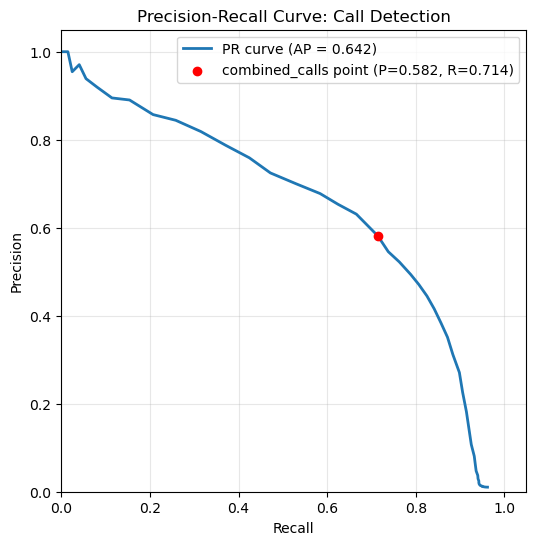
\includegraphics[width=0.3\linewidth]{figures/results/mfcc_5_pr.png}}
    \hspace{1cm}
    \subfloat[10 templates\label{fig:mfcc_10_pr}]{%
        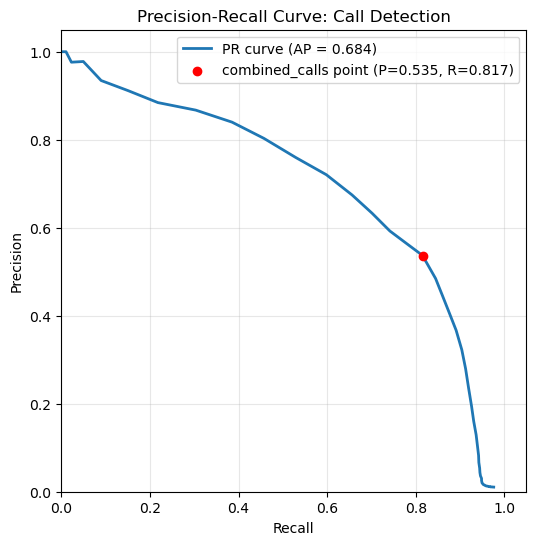
\includegraphics[width=0.3\linewidth]{figures/results/mfcc_10_pr.png}}
    \caption{The PR curves for MFCC}\label{fig:mfcc_pr}
\end{figure}

\begin{figure}[H]
    \centering
    \subfloat[5 templates\label{fig:mfcc_d1_5_pr}]{%
        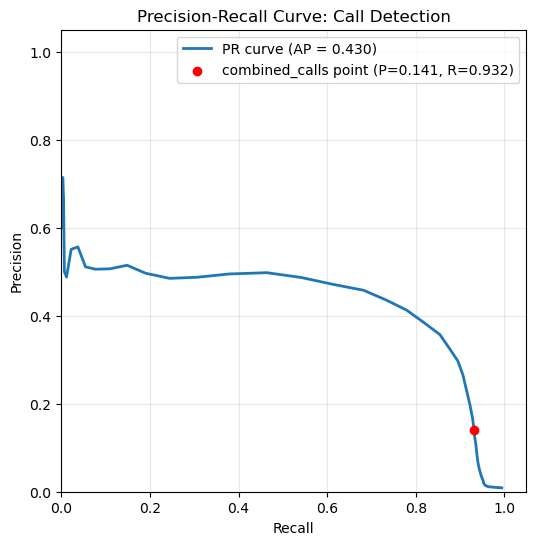
\includegraphics[width=0.3\linewidth]{figures/results/mfcc_d1_5_pr.png}}
    \hspace{1cm}
    \subfloat[10 templates\label{fig:mfcc_d1_10_pr}]{%
        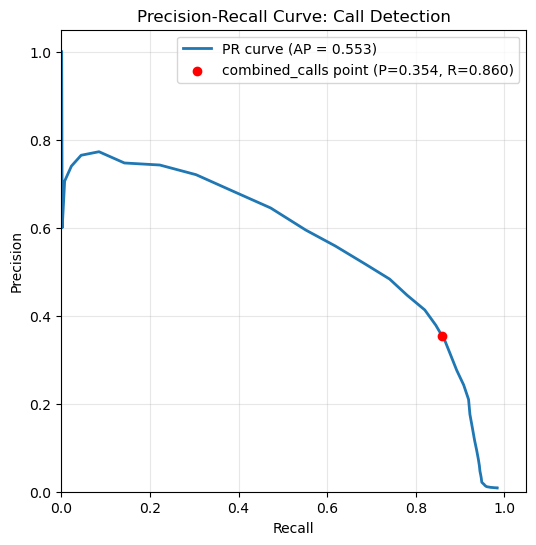
\includegraphics[width=0.3\linewidth]{figures/results/mfcc_d1_10_pr.png}}
    \caption{The PR curves for MFCC with the first derivative added}\label{fig:mfcc_d1_pr}
\end{figure}

\begin{figure}[H]
    \centering
    \subfloat[5 templates\label{fig:mfcc_d2_5_pr}]{%
        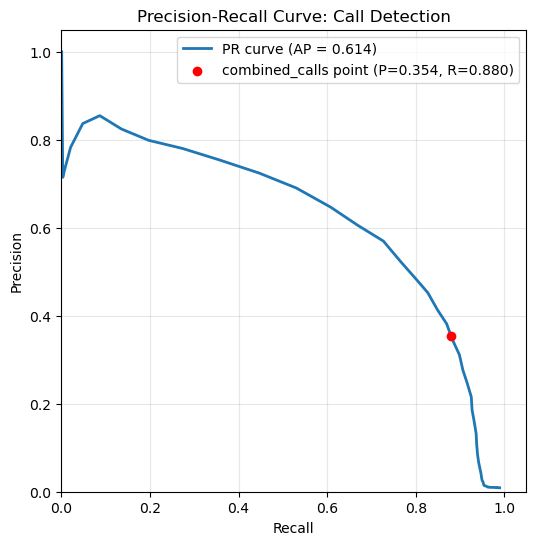
\includegraphics[width=0.3\linewidth]{figures/results/mfcc_d2_5_pr.png}}
    \hspace{1cm}
    \subfloat[10 templates\label{fig:mfcc_d2_10_pr}]{%
        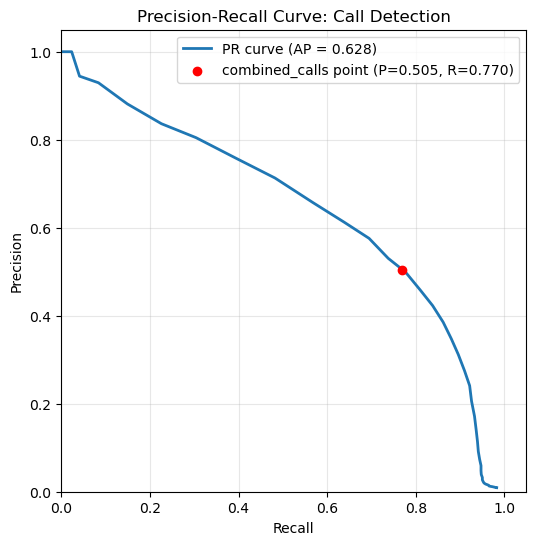
\includegraphics[width=0.3\linewidth]{figures/results/mfcc_d2_10_pr.png}}
    \caption{The PR curves for MFCC with the first and second derivatives added}\label{fig:mfcc_d2_pr}
\end{figure}



\mysection{Experiment 3: LPC Features}{Experiment 3: LPC Features}\label{sec:exp-3-lpc}

\begin{table}[H]
    \caption{Calibration variables chosen via highest F1 for LPC for 5 templates and 10 templates}
    \footnotesize
    \setlength{\tabcolsep}{3pt}
    \centering
    \makebox[\textwidth][c]{%
    \begin{tabular}{ccccccccc}
        \toprule
        \multirow{2}{*}{Number of Temps}
            & \multicolumn{2}{c}{Single Tones}
            & \multicolumn{2}{c}{Multi Tones}
            & \multicolumn{2}{c}{Burst Tonals} 
            & \multirow{2}{*}{Frame Length}
            & \multirow{2}{*}{Vote Fraction}\\
        \cmidrule(lr){2-3} \cmidrule(lr){4-5} \cmidrule(lr){6-7}
            & $F_1$ & Threshold & $F_1$ & Threshold & $F_1$ & Threshold \\
        \midrule
        5  & 0.863 & 0.344 & 0.744 & 0.526 & 0.632 & 0.449 & 0.256 & 0.2\\
        10 & 0.882 & 0.336 & 0.605 & 0.364 & 0.686 &  0.427 & 0.256 & 0.2\\
        \bottomrule
    \end{tabular}\label{tab:lpc_calib_results}
    }
\end{table}

\begin{table}[H]
    \caption{Final test results for LPC for 5 and 10 templates}
    \footnotesize
    \setlength{\tabcolsep}{3pt}
    \centering
    \begin{tabular}{ccccc}
        \toprule
        Number of Temps & Precision & Recall & F1 & Average Precision \\
        \midrule
        5  & 0.190 & 0.930 & 0.316 & 0.697 \\
        10 & 0.351 & 0.916 & 0.508 & 0.772 \\
        \bottomrule
    \end{tabular}\label{tab:lpc_test_results}
\end{table}

\begin{figure}[H]
    \centering
    \subfloat[5 templates\label{fig:lpc_5_pr}]{%
        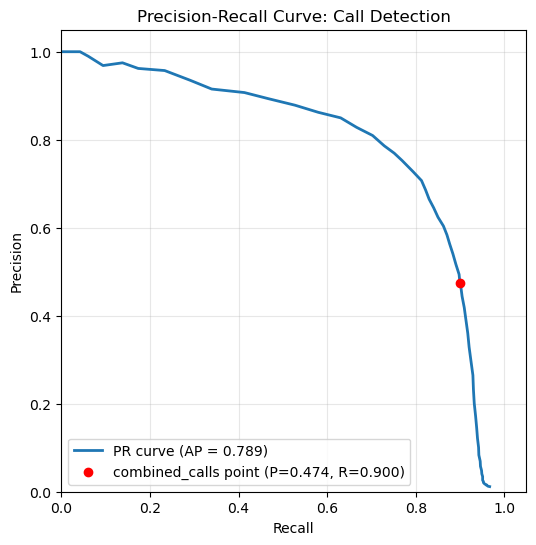
\includegraphics[width=0.3\linewidth]{figures/results/lpc_5_pr.png}}
    \hspace{1cm}
    \subfloat[10 templates\label{fig:lpc_10_pr}]{%
        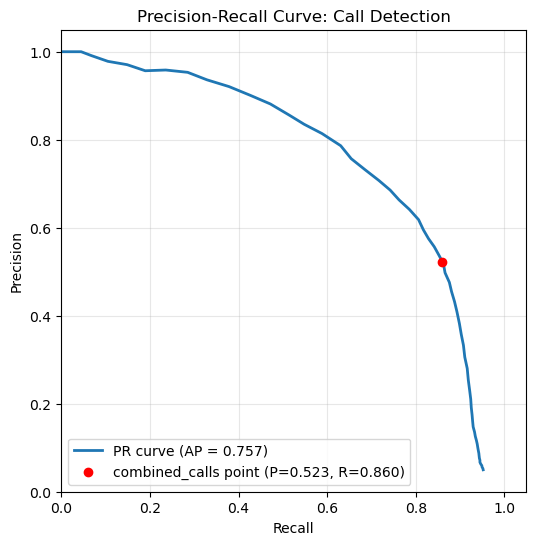
\includegraphics[width=0.3\linewidth]{figures/results/lpc_10_pr.png}}
    \caption{The PR curves for LPC with the first and second derivatives added}\label{fig:lpc_pr}
\end{figure}

\mysection{General Observations}{General Observations}\label{sec:obs}

Considering the low availability of well labeled data to use for the calibration 
stage of this project as well as human error, which was introduced in manual 
selection of calibration and background templates, the varying performance of the 
calibrated thresholds is justified. The lack of data and human error meant that 
a maximum of 10 templates per call type could be used for calibration. It also caused 
a bias in the choices of templates to train on as selecting suitably representative c
templates per call type became difficult. The selection of background templates for 
calibration meant that the class imbalance between calls and background noise 
differed between calibration and testing. The selection of templates and not 
a continuos audio file for calibration also meant that subsequence DTW did not necessarily 
act within the same conditions as testing thus creating another hinderance. 

When looking at printed spectrograms of False Positives detected by the model 
it was found that for both experiments many of these False Positives were actually 
unlabeled calls. This means that the actual precision of the model may be higher 
than the reported amounts. This makes sense as human error was also introduced in 
call labeling, since the known labeled calls were found by previous projects and 
is therefore not necessarily a complete list.

Considering the relitively good performance of the model as well as the unlabeled 
True Positives STFT feature extraction is a good method to use for call detection with 
the DTW algorithm.

